\documentclass{article}
\usepackage[T1]{fontenc}
\usepackage{lmodern}
\usepackage{graphicx}
\usepackage{amsmath,amssymb}
\usepackage[a4paper,margin=2cm]{geometry}
\usepackage[absolute,overlay]{textpos}
\setlength{\TPHorizModule}{1mm}
\setlength{\TPVertModule}{1mm}
\usepackage[indonesian]{babel}
\usepackage{hyperref}
\setlength{\emergencystretch}{2em}
% unit: Halaman 112

\begin{document}

% === Halaman 112 (llm) ===

\begin{itemize}
  \item Sebagai contoh, tinjau 3 rotor yang disederhanakan menjadi hanya 6 huruf alfabet:
\end{itemize}

\vspace{5mm}

\begin{itemize}
  \item Misalkan huruf plainteks D ditekan pada keyboard
  \item Huruf D dienkripsi oleh roto pertama menjadi E
  \item Huruf E menjadi input untuk rotor kedua, dienkripsi menjadi B
  \item Huruf B menjadi input untuk rotor ketiga, dienkripsi menjadi E
  \item Jadi, huruf D dienkripsi menjadi E
\end{itemize}

\vspace{5mm}

\begin{itemize}
  \item Setelah D dienkripsi menjadi E, rotor ketiga bergeser satu huruf.
  \item Jika D dienkripsi kembali, maka hasilnya adalah A
\end{itemize}

\vspace{10mm}

Sumber: \url{https://www.usna.edu/Users/cs/nchamber/courses/ic211/s19/lab/l04/realenigma.html}

% deskripsi: Diagram alur enkripsi huruf D melalui tiga rotor (Rotor 1, Rotor 2, Rotor 3) yang menunjukkan pemetaan huruf dari satu rotor ke rotor berikutnya hingga hasil akhir E.
% bbox normalisasi: [0.0600, 0.1080, 0.9400, 0.9120]
\begin{textblock*}{184.80mm}(12.60mm,32.08mm)
\noindent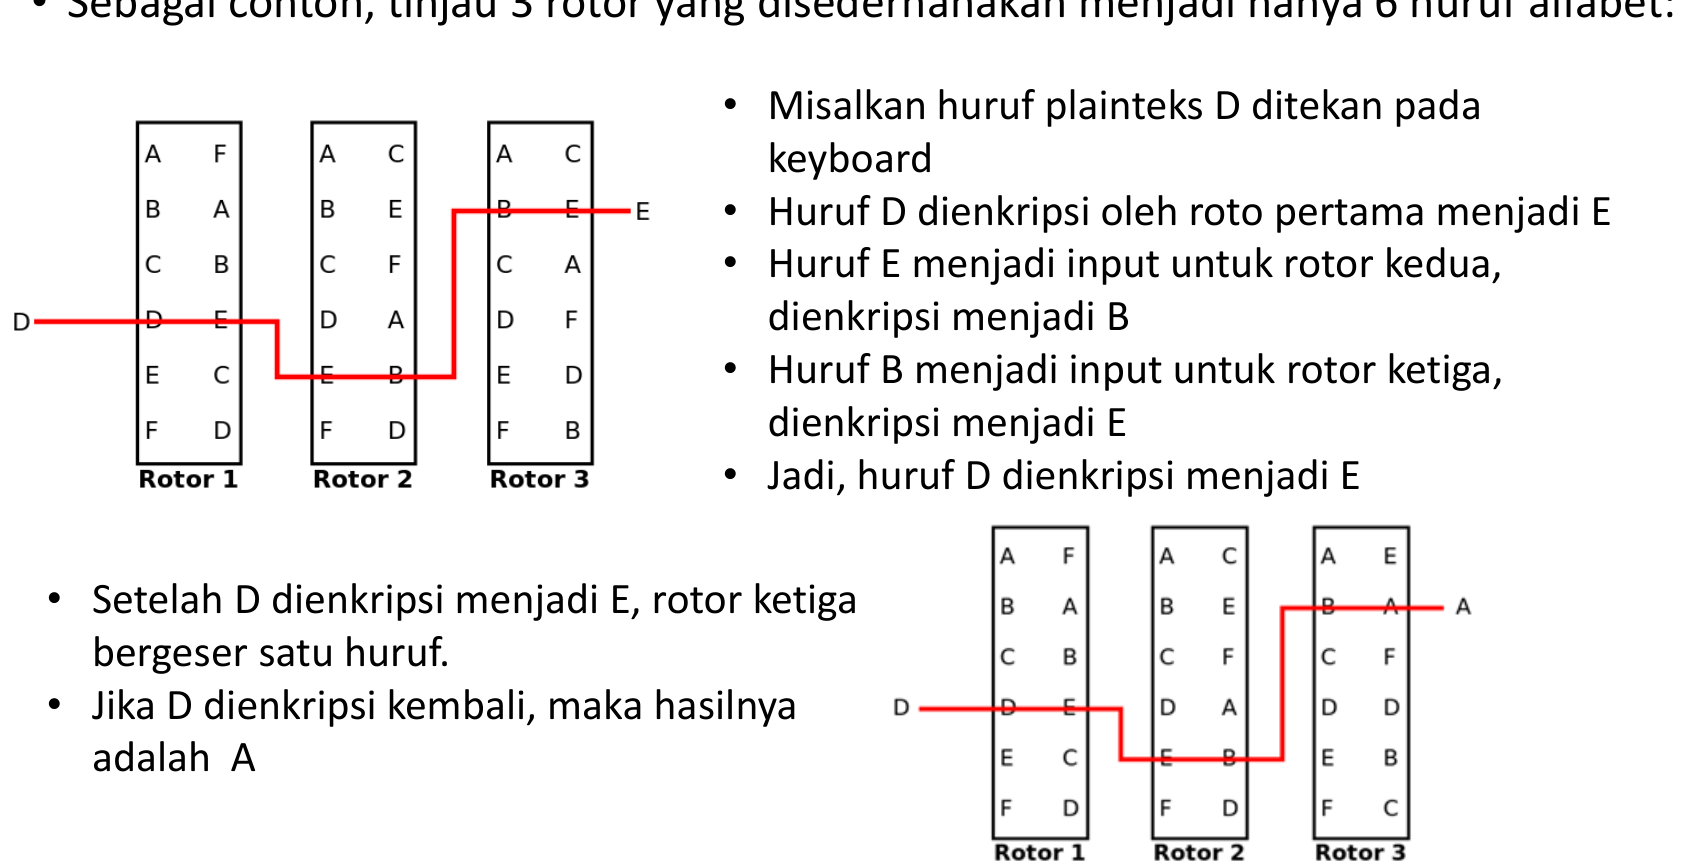
\includegraphics[width=184.80mm,height=238.79mm]{../../images/llm/page_112_img_01.png}%
\end{textblock*}

% deskripsi: Diagram alur enkripsi huruf D setelah rotor ketiga bergeser, menunjukkan pemetaan huruf yang berubah sehingga hasil akhirnya menjadi A.
% bbox normalisasi: [0.5200, 0.6000, 0.8300, 0.9000]
\begin{textblock*}{65.10mm}(109.20mm,178.20mm)
\noindent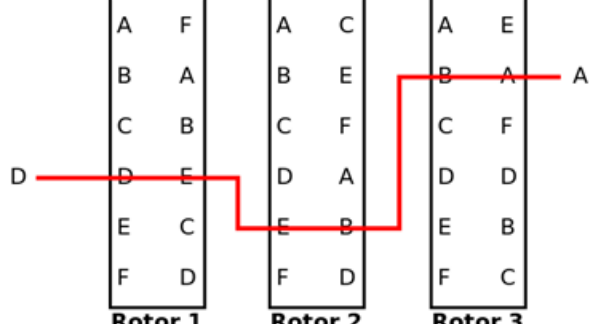
\includegraphics[width=65.10mm,height=89.10mm]{../../images/llm/page_112_img_02.png}%
\end{textblock*}

% bbox perkiraan otomatis: Diagram alur enkripsi huruf D melalui tiga rotor (Rotor 1, Rotor 2, Rotor 3) yang menunjukkan pemetaan huruf dari satu rotor ke rotor berikutnya hingga hasil akhir E.

\end{document}
